\parindent=0em
\section{Definición}
\noindent



Se conoce como realidad mixta o realidad híbrida a la combinación de realidad virtual y realidad aumentada, es decir, a la fusión de añadir información creada por ordenador a un entorno desarrollado tecnológicamente. En esta tecnología el usuario está presente en un mundo que es tanto virtual como físico, destacando principalmente posibilidad de interacción del usuario con el entorno. Se diferencia de la realidad aumentada en que los objetos virtuales si tienen conocimiento de los objetos del mundo físico.
\\\\
Fue en 1994 cuando Paul Milgram y Fumio Kishino definieron el concepto del continuo de la virtualización \cite{ARDisplayofContinuum} indicando que la realidad mixta se define como el entorno que se encuentra en cualquier punto entre los extremos de este (figura~\ref{fig:rvcontinuumfig}).

\begin{figure}[h]
    \centering
    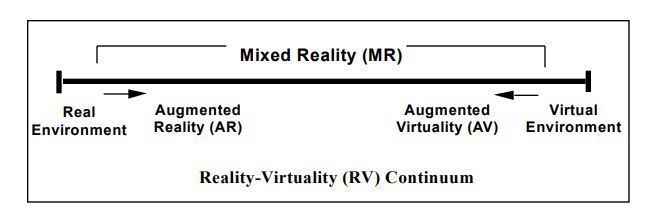
\includegraphics{Images/Estado del arte/rvcontinuum.JPG}
    \caption{Reality-Virtualiy Continuum\textsuperscript{\cite{ARDisplayofContinuum}}}
    \label{fig:rvcontinuumfig}
\end{figure}






